%\documentclass[handout,compress,dvipsnames,pdflatex,beamer]{beamer}
\documentclass[dvipsnames,handout,compress,pdflatex,beamer]{beamer}
%\documentclass[letterpaper,11pt,notitlepage]{article}\usepackage{beamerarticle}
%\usepackage{amsmath}

\usepackage{listings}
\usepackage{url}

\usepackage{color}
\definecolor{myDarkBlue}{rgb}{0.1,0.1,0.4}
\definecolor{myDarkGrey}{rgb}{0.15,0.15,0.15}
\definecolor{myOrange}{rgb}{0.8,0.5,0.0}
\hypersetup{                  		% beamer colors taken from elsewhere
  hyperindex,%				% works with the beetle colour scheme
  colorlinks,%
  linktocpage,%
  plainpages=true,%
  linkcolor=myOrange,%
  citecolor=myDarkGrey,%
  urlcolor=myDarkBlue,%
  pdfstartview=Fit,%
  pdfview={XYZ null null null}%
}


%\newcommand\code{\bgroup\@codex}
%\def\@codex#1{{\normalfont\ttfamily\hyphenchar\font=-1 #1}\egroup}
%\mode<article>{\usepackage[text={6.2in,9in},centering]{geometry}}
%\mode<beamer>{\usetheme{Boadilla}\usecolortheme{seahorse}\usecolortheme{rose}}
%\mode<beamer>{\usetheme[secheader]{Boadilla}\usecolortheme{whale}}
%\mode<beamer>{\usetheme[secheader]{Madrid}\usecolortheme{whale}}

%\mode<beamer>{\setkeys{Gin}{width=\textwidth}}
%\mode<article>{\setkeys{Gin}{width=0.8\textwidth}}

\mode<presentation>{\usetheme{Warsaw}}


\title[C++ for R Programmers]{C++ for R Programmers}


\author[Dirk Eddelbuettel]{Dr.~Dirk Eddelbuettel\\ \scriptsize\url{edd@debian.org}\\ \url{dirk.eddelbuettel@R-Project.org}}

\date[useR! 2012 @ Vanderbilt]{
  { \small 
    Invited Session: 
    \textsl{What other languages should R users know about ?}}\\[20pt] 
  \textsl{useR!} 2012\\ Vanderbilt University \\
  June 14, 2012  }

\begin{document}

%\mode<article>{\maketitle\tableofcontents}

\mode<presentation>{\frame{\titlepage}}

%\mode<presentation>{\frame{\frametitle{Outline}\tableofcontents[pausesections,hideallsubsections]}}

\section[C++?]{Why C++?}

\subsection{Overview}

\begin{frame}

  \begin{figure}
    
\includegraphics[scale=0.55]{images/there-be-dragons-map.jpg}
  \end{figure}

\end{frame}

\begin{frame}
  \frametitle{So ``Why C++'' ?}

  \pause
  \begin{itemize}[<+->]
  \item Asking Google leads to 51,600,000 hits. 
  \item No, I didn't read all of those.
  %\item I did not read all of them.
  %\item Some lead to people at most one degree of
  %  separation away from the audience like John D.~Cook.
  \item \href{http://en.wikipedia.org/wiki/C\%2B\%2B}{Wikipedia} starts with
    \emph{C++ (pronounced "cee plus plus") is a statically typed,
      free-form, multi-paradigm, compiled, general-purpose, powerful
      programming language.}  
  \item We could spend this session discussing just that sentence.
  \item C++ is industrial-strength, widely-used, vendor-independent and
    \emph{still evolving}.
  \item In science and research, it is one of the most widely-used
    languages.  If there is something you want to use or connect to, it
    probably has a C/C++ API.
  \item As a widely used language it also has good tool support (debuggers,
    [memory] profilers, code analysis).
  \end{itemize}
\end{frame}

\subsection{Federation}
\begin{frame}
  \frametitle{A popular view on ``What C++ is''}
  \framesubtitle{From Scott Meyers highly-regarded``Effective C++''}

  \pause

  Item 1:   \emph{``View C++ as a federation of languages''}

  \pause

  \begin{enumerate}[<+->]
  \item \emph{C} provides a rich inheritance and interoperability as Unix, Windows,
    ... are all build on C.
  \item \emph{Object-Oriented C++} just to provide endless discussions about
    exactly what OO is or should be (and R really helps here having
    three different ones to offer :-/ ).
  \item \emph{Templated C++} which is mighty powerful; template meta
    programming unequalled in other languages.
  \item \emph{The STL} which is a specific template library which is powerful but
    has its own conventions.
  \end{enumerate}
  
  \pause And C++11 adds many more goodies that could be called a fifth language.
\end{frame}

\section[With R]{Why C++ with R?}
\subsection{Mixing}
\begin{frame}
  \frametitle{\textsl{Barbells not bullets}}
  \begin{itemize}[<+->]
  \item ``Barbell'' portfolios mean those comprised of both long and short
    duration bonds -- as opposed to ``bullet'' portfolio concentrated at one
    (middle) duration. 
  \item I feel language choice is similar:  It is rare to have one single
    solution for all problems. Python may be close;  Julia may get there too.
  \item But I am a realist, and I have \emph{never} been on a project or
    team that was single-language, single-solution.
  \item In practice, people will always mix.  %John Chambers has made that point eloquently too.
  %\item 
    So let's face this head-on and pick tools \emph{which mix well}.  
  \item It so happens that I think R and C++ mix well via Rcpp and RInside.
  \end{itemize}
\end{frame}

\subsection{Interface}
\begin{frame}
  \frametitle{John Chambers agrees -- and shares a ``vision'' from 1976}
  %\framesubtitle{A ``interface'' vision from 1976}

  \begin{figure}
    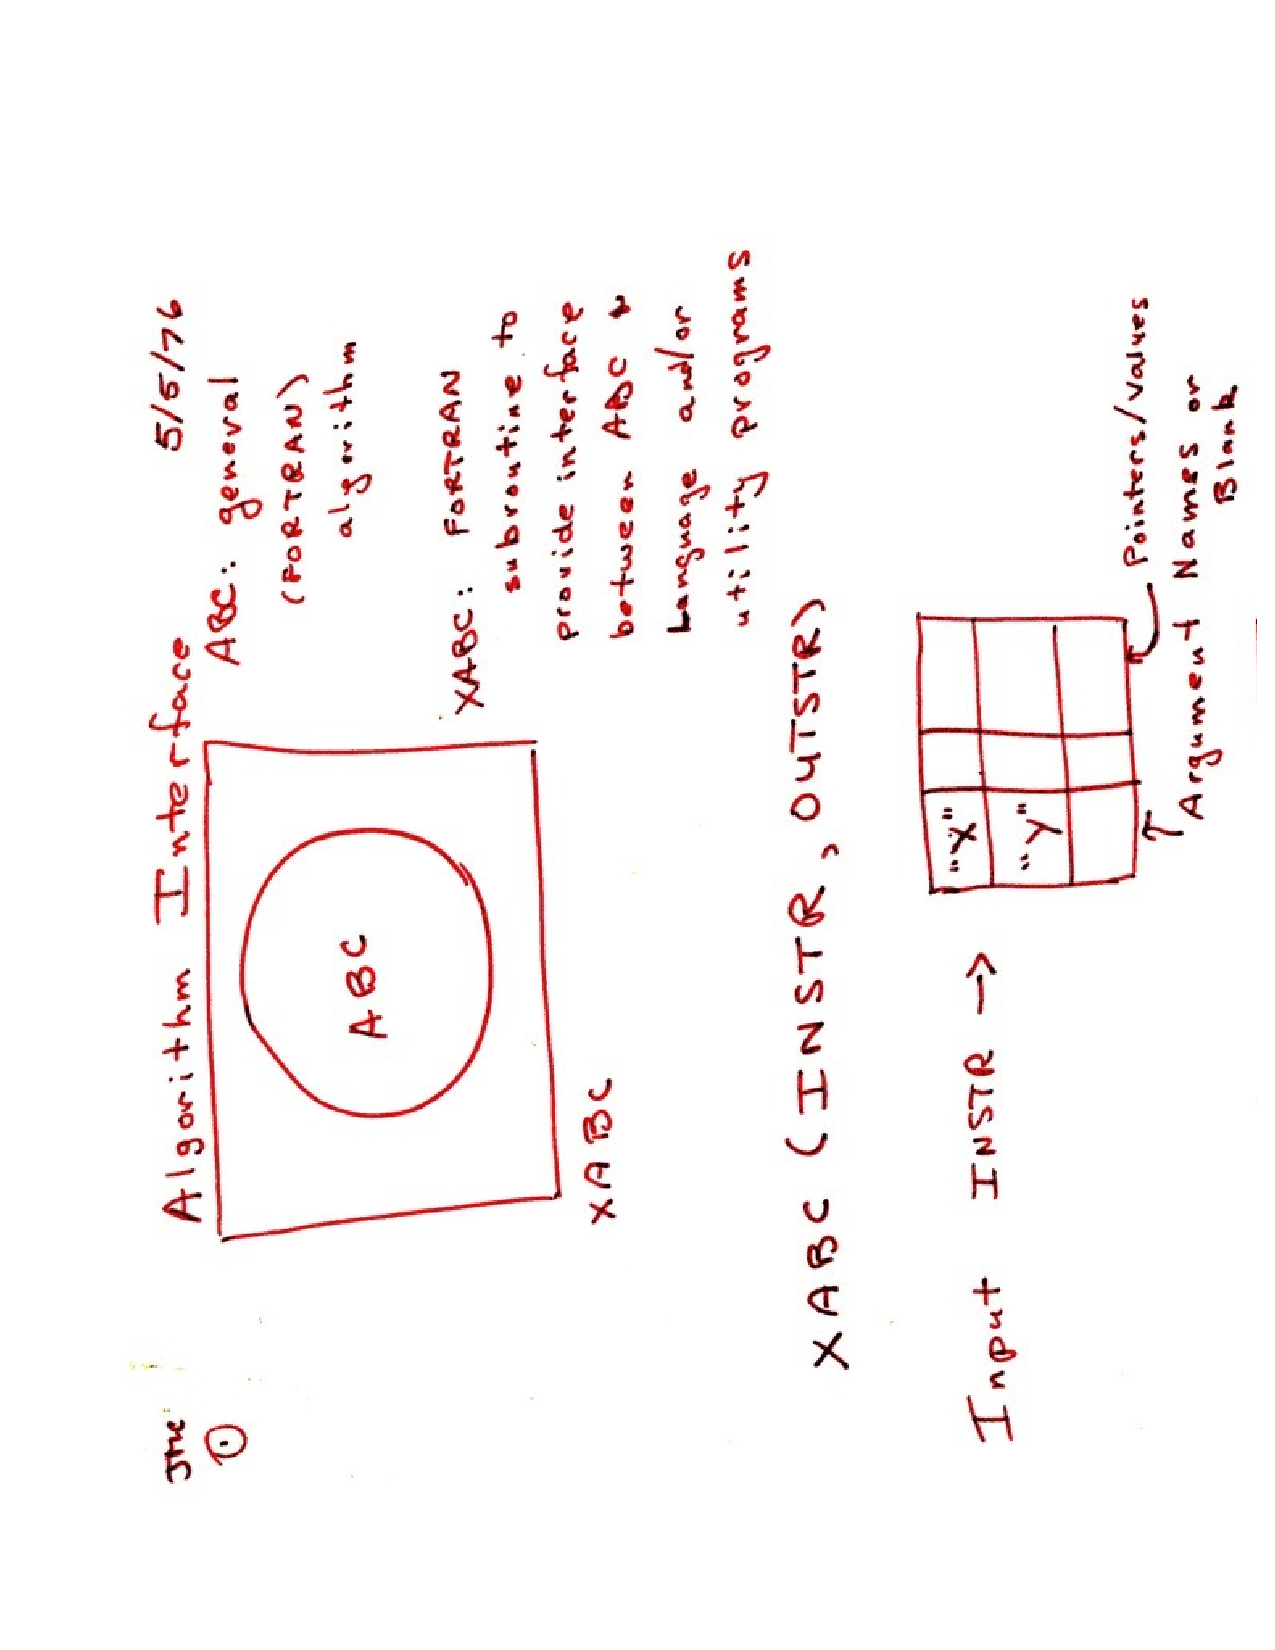
\includegraphics[scale=0.3,angle=270]{images/Chambers2010_Page6.pdf}
  \end{figure}

  \medskip \footnotesize Source: John Chambers' talk at Google, 2010.
\end{frame}

\subsection{Interchange}
\begin{frame}
  \frametitle{Sending R objects back and forth}
  \framesubtitle{Possible with R's API, easier with Rcpp}
  \begin{itemize}[<+->]
  \item Essentially, any R object is represented internally as a SEXP.
  \item The \texttt{.Call} interface lets you send SEXPs back and forth.
  \item SEXP can be nested just like R objects: lists of lists of ...
  \item Rcpp makes the interchange of R objects a little easier than the
    plain C API for R. 
  \item ``Empirically speaking'', 68 CRAN packages (as
    of 3 June 2012) using Rcpp seem to agree.
  \item This makes Rcpp the most widely used foreign-language interface
    package for R (as it overtook rJava recently). 
    % Of course, there is the plain C API...
  \end{itemize}
\end{frame}

\iffalse
\section{Competition}

\subsection{Python}
\begin{frame}
  \frametitle{Python}
  %\frametitle{  \emph{Trust me, Mogli....}  --  Seriously?}
  \pause

  \begin{figure}
    %
\includegraphics[scale=0.8]{images/Mowglikaa2.jpg}
    
\includegraphics[scale=0.6]{images/jungle-book-kaa.jpg}
  \end{figure}

  \smallskip
  
  \pause
  \emph{Trust me, Mogli....}   Seriously?
\end{frame}


\subsection{Julia}
\begin{frame}
  \frametitle{Julia}
  \pause

  \begin{figure}
    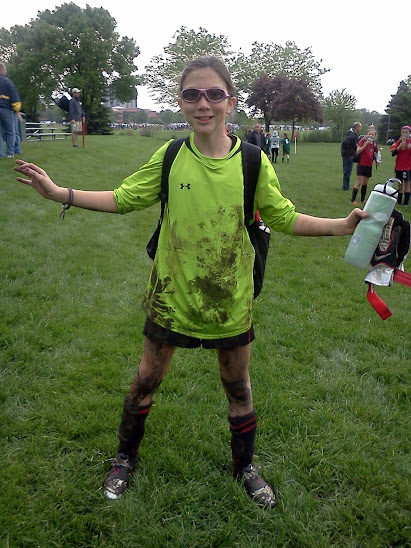
\includegraphics[scale=0.3]{images/JEasGoalie.jpeg}
  \end{figure}

  \medskip

  My Julia -- and until I find a matching language named after my other
  daughter Anna ...

\end{frame}
\fi

\section{Shootout}
\begin{frame}
  \frametitle{Shootout and C++ / Rcpp based solutions}

  \begin{enumerate}[<+->]
  \item Gibbs Sampler example:  I don't actually have much to add here which
    wasn't in the earlier blog posts.
  \item Metropolis example:  Whit Armstrong covered that in his recent
    rcppbugs package.
  \item Chris will cover both in the Python part.
  \end{enumerate}
\end{frame}


\section{Outlook}
\begin{frame}
  \frametitle{C++11: The future}
  \framesubtitle{These are interesting times}

  \begin{itemize}[<+->]
  \item Arguably, new standard C++11 makes C++ a new language.
  \item LLVM/Clang++ offers venues for static / dynamic code
    analysis and emergence of new tools.
  \item Lots of very promising changes---while maintaining full
    compatibility and 
    \begin{itemize}
      \item still being the \emph{fastest possible language} 
      \item while having \emph{zero overhead}.
    \end{itemize}
  \end{itemize}
\end{frame}  

\section{Resources}
\begin{frame}
  \frametitle{C++ Resources}
  \begin{itemize}
  \item The book / website
    \href{http://www.icce.rug.nl/documents/cplusplus/}{C++ Annotations} by
    Brokken is very good, current and frequently updated.
  \item StackOverflow has a very good curated
    \href{http://stackoverflow.com/questions/388242/the-definitive-c-book-guide-and-list}{definite C++ book list}
  \item Wikipedia is thorough as usual on
    \href{http://en.wikipedia.org/wiki/C\%2B\%2B}{C++} as well as 
    \href{http://en.wikipedia.org/wiki/C\%2B\%2B11}{C++11}
  \item R and C++: 
    \href{http://dirk.eddelbuettel.com/code/rcpp.html}{Rcpp page}, 
    \href{http://cran.r-project.org/package=Rcpp}{CRAN page} and 
    \href{http://www.jstatsoft.org/v40/i08/}{JSS paper}
  \item Lastly, thanks to JJ, two pointers to two very recent talks: 
    \begin{itemize}
    \item Herb Sutter on \href{http://channel9.msdn.com/Events/Lang-NEXT/Lang-NEXT-2012/-Not-Your-Father-s-C-}{(Not your father's) C++}
    \item Chandler Carruth on \href{http://channel9.msdn.com/Events/GoingNative/GoingNative-2012/Clang-Defending-C-from-Murphy-s-Million-Monkeys}{Clang Defending C++ from Murphy's Million Monkeys}
    \end{itemize}
  \end{itemize}
\end{frame}

% Sutter: (Not your Father's) C++
% http://channel9.msdn.com/Events/Lang-NEXT/Lang-NEXT-2012/-Not-Your-Father-s-C-

% What makes ISO C++11 "feel like a new language"? What things that we know
% about past C++ do we need to unlearn? Why is C++ designed the way it is –
% historically, and in C++11? Finally, what is the difference between managed
% and native languages anyway, and when is each applicable? This talk gives an
% overview and motivation of modern C++ and why it's clean, safe, and fast – as
% clean to code in and as type-safe as any modern language, and more than ever
% the king of "fast."


% Chandler Carruth
% http://channel9.msdn.com/Events/GoingNative/GoingNative-2012/Clang-Defending-C-from-Murphy-s-Million-Monkeys

% Were we to craft a Lenox Globe of programming languages, C++ might be
% followed by a famous cautionary phrase: Here Be Dragons. The language can be
% complex and daunting to programmers who are often shouldered with the task of
% writing large, complex programs. Those millions of code monkeys need help to
% resist Murphy's siren song and navigate C++'s treacherous waters of memory
% corruption and concurrency bugs.
 
% Clang is a C++ compiler platform that tries to address these challenges
% (among others) across the spectrum of development activities. It provides
% fantastic diagnostics, static and dynamic program analysis, advanced
% rewriting and refactoring functionality, and language extensibility. Together
% with improvements to the language in C++11 these help programmers cope with
% today's code and write better code tomorrow. Clang also makes it easier than
% ever before to evolve and evaluate new language features and extensions to
% make C++ itself better.
 
% Through this talk I'll give some background on the Clang compiler, what it
% does today to make writing C++ better, and how we're using it to help shape
% the C++ language going forward.

\end{document}

%%% Local Variables: 
%%% mode: latex
%%% TeX-master: t
%%% End: 
